%%%%%%%%%%%%%%%%%%%%%%%%%%%%%%%%%%%%%%%%%%%%%%%%%%%%%%%%%%%%%%%%%%%%
%%%
%%% Macros 
%%% Curso de Especialização em Sistemas Eletrônicos para Controle
%%% Faculdade SENAI Anchieta - São Paulo - SP
%%% José William Rodrigues Pereira 
%%% Outubro / 2015
%%%
%%%%%%%%%%%%%%%%%%%%%%%%%%%%%%%%%%%%%%%%%%%%%%%%%%%%%%%%%%%%%%%%%%%%

%%%------------------------------------ Dados
\def\autor#1{\gdef\autor{#1}}
\def\nome#1{\gdef\nome{#1}}
\def\ultimonome#1{\gdef\ultimonome{#1}}
\def\titulo#1{\gdef\titulo{#1}}
\def\subtitulo#1{\gdef\subtitulo{#1}}
\def\curso#1{\gdef\curso{#1}}
\def\instituicao#1{\gdef\instituicao{#1}}
\def\sigla#1{\gdef\sigla{#1}}
\def\unidadeacademica#1{\gdef\unidadeacademica{#1}}
\def\grau#1{\gdef\grau{#1}}
\def\tipodotrabalho#1{\gdef\tipodotrabalho{#1}}
\def\orientador#1{\gdef\orientador{#1}}
\def\torientador#1{\gdef\torientador{#1}}
\def\coorientador#1{\gdef\coorientador{#1}}
\def\tcoorientador#1{\gdef\tcoorientador{#1}}
\def\cidade#1{\gdef\cidade{#1}}
\def\ano#1{\gdef\ano{#1}}
\def\npaginas#1{\gdef\npaginas{#1}}
\def\CDU#1{\gdef\CDU{#1}}
\def\areas#1{\gdef\areas{#1}}
\def\examinadorum#1{\gdef\examinadorum{#1}}
\def\texaminadorum#1{\gdef\texaminadorum{#1}}
\def\examinadordois#1{\gdef\examinadordois{#1}}
\def\texaminadordois#1{\gdef\texaminadordois{#1}}
\def\data#1{\gdef\data{#1}}
\def\palavraschave#1{\gdef\palavraschave{#1}}
\def\keywords#1{\gdef\keywords{#1}}

%%%%------------------------------------ Configuração das Páginas
\newcommand{\configuramargens} %%% Define margens
{
  \usepackage[width=210.00mm, height=297.00mm, 
			  left=3.00cm,    right=2.00cm, 
			  top=3.00cm,     bottom=2.00cm] {geometry}
}

%%%------------------------------------ Fonte
%\renewcommand{\familydefault}{\sfdefault} % sans font
\renewcommand{\familydefault}{\rmdefault}  % roman font


%%%------------------------------------ Formatação de Capitulo
\titleformat{\chapter}
  {\Large\bfseries}
  {}
  {0pt}
  {\huge}

%%%------------------------------------ Capa
\newcommand{\capa}
{
  \begin{titlepage}
    \thispagestyle{empty}
    \begin{center}
      \textsc{\instituicao} 		\\[5.0cm]
%      \textsc{\unidadeacademica}	\\[0.0cm]
%      \textsc{Curso de \curso}		\\[4.0cm]
      \textsc{\autor}			\\[5.0cm]
      \textsc{\titulo}			\\[0.0cm]
      \textsc{\subtitulo}               \\[0.4cm]
      \vfill
      \textsc{\cidade}			\\[0.0cm]
      \textsc{\ano}			\\[0.0cm]
    \end{center}
  \end{titlepage}
}
%%%------------------------------------ Natureza
\newcommand{\natureza}
{
  \begin{flushright}
    \thispagestyle{empty}
    \begin{minipage}{0.54\textwidth}
    {
      \tipodotrabalho apresentada ao \instituicao 
      como requisito para 
      obtenção do grau de \grau em \curso
    } 				\\[0.4cm]
    Orientador:   \torientador    \orientador \\
%    Coorientador: \tcoorientador  \coorientador
    \end{minipage}
  \end{flushright}
}
%%%------------------------------------ Folha de Rosto
\newcommand{\folhaderosto}
{
  \begin{titlepage}
    \begin{center}
      \textsc{ }		\\[5.0cm]
      \textsc{\autor}		\\[5.0cm]
      \textsc{\titulo}		\\[0.0cm]
      \textsc{\subtitulo}       \\[4.0cm]
      \natureza
      \vfill
      \textsc{\cidade}		\\[0.0cm]
      \textsc{\ano}		\\[0.0cm]
    \end{center}
  \end{titlepage}
}
%%%------------------------------------ Ficha Catalográfica
\newcommand{\fichacatalografica}
{

\begin{figure}[!h]
\vspace{13cm}
\center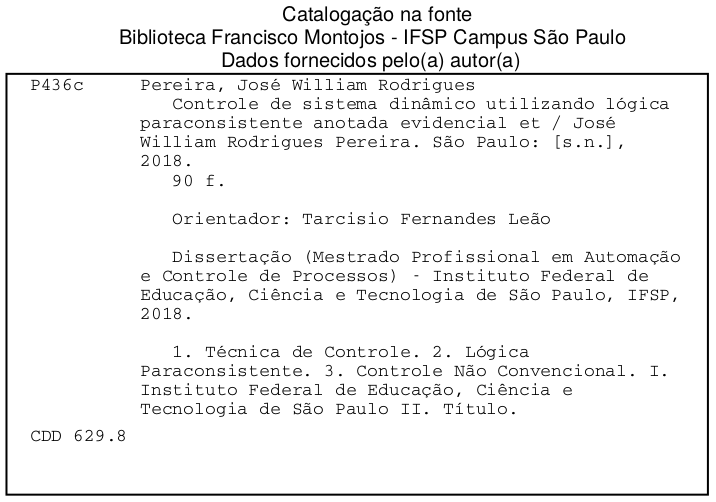
\includegraphics[scale=0.6]{./imagens/fichaCatalog.png}
\end{figure}


%  \begin{titlepage}
%    \vfil\null
%    \vfill
%    \fbox
%    {
%      \begin{tabular}{p{14.0cm}}
%        P492c \ultimonome, \nome \\
%	\hspace{1cm} \begin{minipage}{0.8\textwidth}
%             \hspace{1cm} \titulo \subtitulo\ / \nome\ \ultimonome\ , - - \cidade , \ano .\\
%            \npaginas f. : il   					\\
%									\\
%	    \hspace{1cm} Orientador: \orientador . 			\\
%	    \hspace{1cm} \grau (\curso ) - - 				\\
%	    \hspace{1cm} \instituicao , \ano .				\\
%									\\
%            \areas . I. Leão, Tarcisio Fernandes. II. Título. 		\\
%									\\
%	    \begin{flushright}
%            \hfill CDD \CDU
%	    \end{flushright}
%        \end{minipage}
%      \end{tabular} 
%    }  
% \end{titlepage}
}
%%%------------------------------------ Folha de Aprovação
\newcommand{\folhadeaprovacao}
{

\begin{figure}[!h]
\center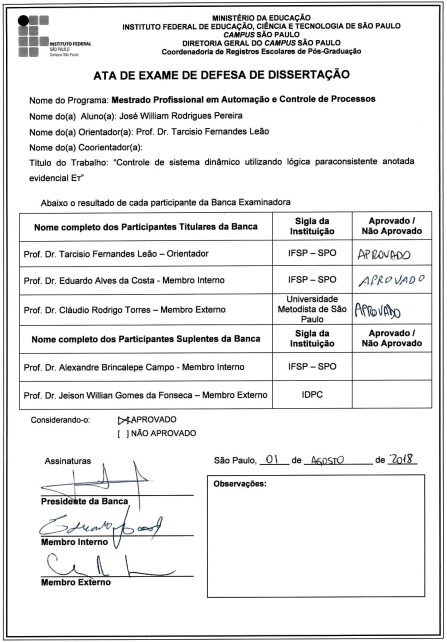
\includegraphics[scale=1.05]{./imagens/ataJWRP.png}
\end{figure}


%  \begin{titlepage}
%    \thispagestyle{empty}
%    \begin{center}
%      \textsc{\autor}
%      \vfill
%      \textsc{ \titulo } \\
%      \textsc{ \subtitulo }
%      \vfill
%    \end{center}
%    \natureza
%    \vfill
%    \centering Aprovado pela banca examinadora em \data \\
%    \vfill
%    \begin{center}
%      {\large\bfseries BANCA EXAMINADORA }\\
%      \vfill
%      \rule{9.0cm}{0.1mm} \\
%      {\torientador \orientador  }\\
%      {Orientador } \\
% %     \vfill
% %     \rule{9.0cm}{0.1mm} \\
% %     {\tcoorientador \coorientador} \\
% %     {Coorientador} \\
%      \vfill
%      \rule{9.0cm}{0.1mm} \\
%      {\texaminadorum \examinadorum }\\
%      \vfill
%      \rule{9.0cm}{0.1mm} \\
%      {\texaminadordois \examinadordois}
%    \end{center}
%  \end{titlepage}
}
%%%------------------------------------ Dedicatória
\newcommand{\dedicatoria}[1]
{
  \begin{titlepage} 
    \thispagestyle{empty}
    \titlepage
    \begin{center}%
        \huge \textbf{Dedicatória}
    \end{center}%
    \null
    \hspace{1cm} #1
    \endtitlepage
  \end{titlepage}

%  \begin{titlepage}
%  \thispagestyle{empty}
%  \hspace{1cm}
%  \vfill
%  \begin{flushright}
%    \begin{minipage}{0.6\textwidth}
%    \textrm
%    {
%      \textit
%      {
%	#1
%      }
%    }    
%    \end{minipage}
%  \end{flushright}
%  \end{titlepage}
}

%%%------------------------------------ Agradecimentos
\newcommand{\agradecimentos}[1]
{
  \begin{titlepage} 
    \thispagestyle{empty}
    \titlepage
    \begin{center}%
        \huge \textbf{Agradecimentos}
    \end{center}%
    \null
    \hspace{1cm} #1
    \endtitlepage
  \end{titlepage}
}

%%%------------------------------------ Epígrafe
\newcommand{\epigrafe}[1]
{
  \begin{titlepage}
    \thispagestyle{empty} 
    \hspace{1cm}
    \vfill
    \begin{flushright}
      \begin{minipage}{0.6\textwidth}
      \textrm
      {
        \textit
        {
	    #1
        }
      }    
      \end{minipage}
    \end{flushright}
  \end{titlepage}
}

%%%------------------------------------ Resumo
\newcommand{\resumo}[1]
{
  \begin{titlepage} 
    \titlepage  
    \thispagestyle{empty}
    \begin{center}%
        \huge \textbf{Resumo}
    \end{center}%
    \null
    #1

    \textbf{\\PALAVRAS-CHAVE:} \palavraschave
    \endtitlepage
  \end{titlepage}
}
%-------------------------------------- Abstract
\newcommand{\resumolinguaestrangeira}[1]
{
  \begin{titlepage} 
    \titlepage
    \thispagestyle{empty}  
    \begin{center}%
        \huge \textbf{Abstract}
    \end{center}%
    \null  
    \hspace{1cm} 
    #1

    \textbf{\\KEYWORDS:} \keywords
    \endtitlepage
  \end{titlepage}
}
%-------------------------------------- Sumário
\newcommand{\sumario}
{
    \tableofcontents
    \thispagestyle{empty}
}
%-------------------------------------- Lista de figuras
\newcommand{\listadefiguras}
{
  \listoffigures
  \thispagestyle{empty}
}
%-------------------------------------- Lista de tabelas
\newcommand{\listadetabelas}
{
  \listoftables
  \thispagestyle{empty}
}

%-------------------------------------- Lista de abreviaturas e siglas
\newcommand{\abreviatura}[2]
{
  \nomenclature{#1}{#2}
  #1
}
\newcommand{\listadeabreviaturasesiglas}
{
  \renewcommand{\nomname}{Lista de abreviaturas e siglas}
  \printnomenclature[5em]
  \thispagestyle{empty}	
}
%%%------------------------------------ Citação
\newcommand{\citacao}[1]
{
  \begin{flushright}
    \begin{minipage}{12cm}
      \footnotesize #1
    \end{minipage}
    \vspace{12pt}
  \end{flushright}
}

%--------------------------------------
%--------------------------------------


%--------------------------------------
%-------------- Estilo do Codigo Fonte
\definecolor{verde}{rgb}{0.25,0.5,0.35}
\definecolor{jpurple}{rgb}{0.5,0,0.36}

\lstset{
  language=C,
  basicstyle=\ttfamily\small,
  keywordstyle=\color{blue},
  stringstyle=\color{verde},
  commentstyle=\color{red},
  extendedchars=true,
  showspaces=false,
  showstringspaces=false,
  numbers=left,
  numberstyle=\small,
  breaklines=true,
  backgroundcolor=\color{green!10},
  breakautoindent=true,
  captionpos=b,
  xleftmargin=0pt,
}

%--------------------------------------:w



